% Author: Dominik Harmim <harmim6@gmail.com>


\documentclass[a4paper, 11pt]{article}


\usepackage[utf8]{inputenc}
\usepackage[british]{babel}
\usepackage[left=2cm, top=3cm, text={17cm, 24cm}]{geometry}
\usepackage{times}
\usepackage{graphicx}
\usepackage{amsmath}
\usepackage{enumerate}
\usepackage[table]{xcolor}
\usepackage{float}
\usepackage{multirow}


\begin{document}


	%%%%%%%%%%%%%%%%%%%%%%%%%%%%%%%% Title page %%%%%%%%%%%%%%%%%%%%%%%%%%%%%%%%
	\begin{titlepage}
		\begin{center}
			
\includegraphics[width=0.5\linewidth]{inc/Bangor_logo.pdf} \\

			\vspace{\stretch{0.382}}

			\LARGE{ICP-2011 -- Computer Networks} \\
			\Huge{\textbf{Assignment -- Review Questions}}

			\vspace{\stretch{0.618}}
		\end{center}

		{\Large
			\today
			\hfill
			Dominik Harmim (eeub8c)
		}
	\end{titlepage}



	%%%%%%%%%%%%%%%%%%%%%%%%%%%%%%%% Answers %%%%%%%%%%%%%%%%%%%%%%%%%%%%%%%%
	\section*{Answers}

	\begin{enumerate}
		\item % 1.
			\textbf{Pure Time Division Multiplexing (TDM)} -- The time slots are allocated on a constant basis.
			This means that user 1 always gets time slot 1, user 2 always gets time slot 2, and so no.
			Provided bandwidth is not used efficiently. There is guaranteed transmission path.

			\textbf{Statistical Time Division Multiplexing (STDM)} -- Allocates bandwidth to each user on the basis
			of demands and needs. A user uses time slots only when they are actually transmitting data.
			When a user is not sending data, no time slots are allocated to it, and other users that
			are sending data can use these time slots. Time slots are allocated statistically.

			$ \text{raw data rate of the user} = \boldsymbol{B \cdot \frac{1}{T}\,\text{\textbf{b}}} $ \\
			$ \text{raw data rate of the entire TDM channel} = \boldsymbol{B \cdot N \cdot \frac{1}{T}\,\text{\textbf{b}}} $

			$ \text{user A transmission bandwidth} = 10 \cdot 2 = \boldsymbol{20\,\text{\textbf{Mb/s}}} $ \\
			$ \text{user C transmission bandwidth} = \frac{10}{2} = \boldsymbol{5\,\text{\textbf{Mb/s}}} $

		\item % 2.
			Error digit correction in given information matrix with column/row even parity digits:
			\begin{table}[H]
				\centering
				\begin{tabular}{c c c c | c}
					0 & 0 & 1 & 0 & \\ \hline
					0 & {\color{red} 1} & 1 & 1 & 1 \\
					0 & 1 & 1 & 0 & 0 \\
					1 & 0 & 0 & 0 & 1 \\
					1 & 0 & 1 & 1 & 1 \\
				\end{tabular}
				\caption{Information matrix with column/row even parity digits}
				\label{table:information_parity_matrix}
			\end{table}

			Parity checking-based error correction technique fails when even number of errors occur.

		\item % 3.
			Data network architecture diagram:
			\begin{figure}[H]
				\centering
				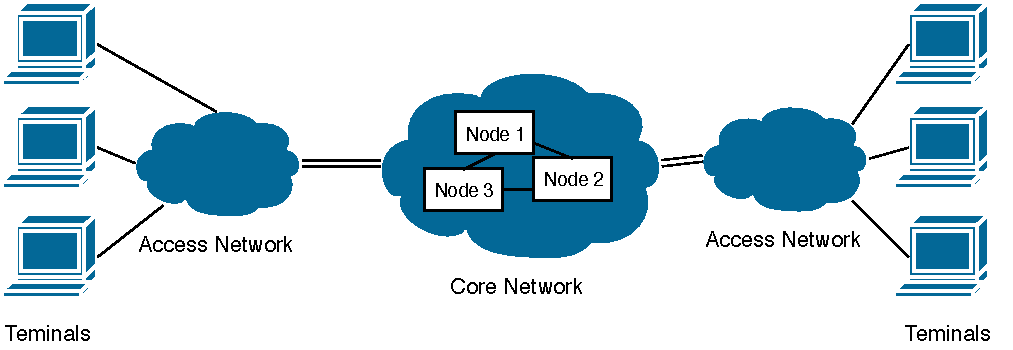
\includegraphics[width=0.7\linewidth]{inc/data_network_architecture.pdf}
				\caption{Data Network Architecture}
				\label{figure:data_network_architecture}
			\end{figure}

			\textbf{Communication protocol} -- Set of rules and procedures describing exchange the information
			within networks. Protocols enables devices to communicate by using set of rules.

			\textbf{Communication architecture} -- Describes special functions that the computer hardware and software
			must perform to allow application programs to communicate with the outside world.
			Communication architecture is based on communication protocol.

		\item % 4.
			OSI reference model layers:
			\begin{enumerate}[1]
				\item % 1
					Physical Layer
					\begin{description}
						\item vi) Mechanical, electrical and functional interface.
					\end{description}

				\item % 2
					Data Link Layer
					\begin{description}
						\item i) Error correction and re-transmission.
						\item iv) Responsibility for carrying frames between adjacent nodes.
						\item vii) Flow control.
						\item viv) Three packet switching technologies including X.25, Frame Relay and ATM.
					\end{description}

				\item % 3
					Network Layer
					\begin{description}
						\item iii) Route determination.
						\item viv) Three packet switching technologies including X.25, Frame Relay and ATM.
					\end{description}

				\item % 4
					Transport Layer
					\begin{description}
						\item i) Error correction and re-transmission.
						\item vii) Flow control.
						\item viii) Reliable process-to-process message delivery.
					\end{description}

				\item % 5
					Session Layer
					\begin{description}
						\item ii) Establishing and monitoring an entire communication connection between users.
					\end{description}

				\item % 6
					Presentation Layer

				\item % 7
					Application Layer
					\begin{description}
						\item v) Communicates directly with user’s application program.
					\end{description}
			\end{enumerate}

		\item % 5.
			Diagram shows content of packets when computer A sends data to computer D:
			\begin{figure}[H]
				\centering
				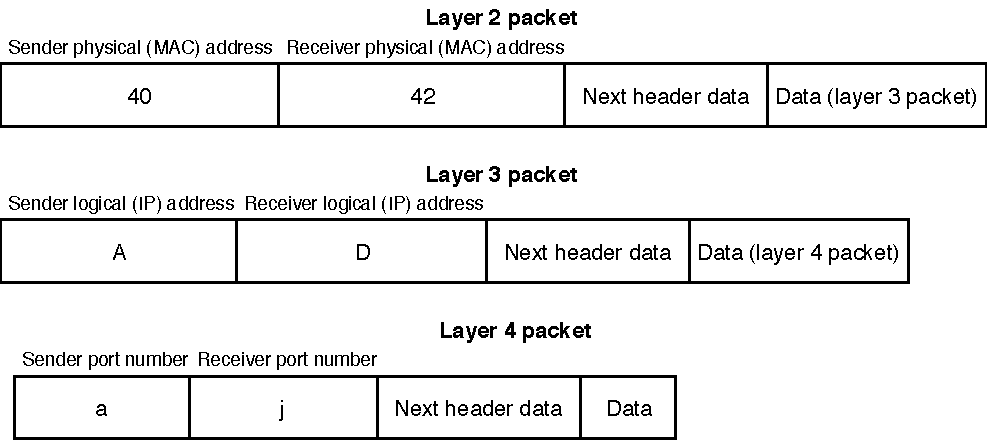
\includegraphics[width=0.7\linewidth]{inc/layer_packets_a_to_d.pdf}
				\caption{Computer A sends data to computer D}
				\label{figure:layer_packets_a_to_d}
			\end{figure}

			Diagram shows content of packets when computer D sends data to computer A:
			\begin{figure}[H]
				\centering
				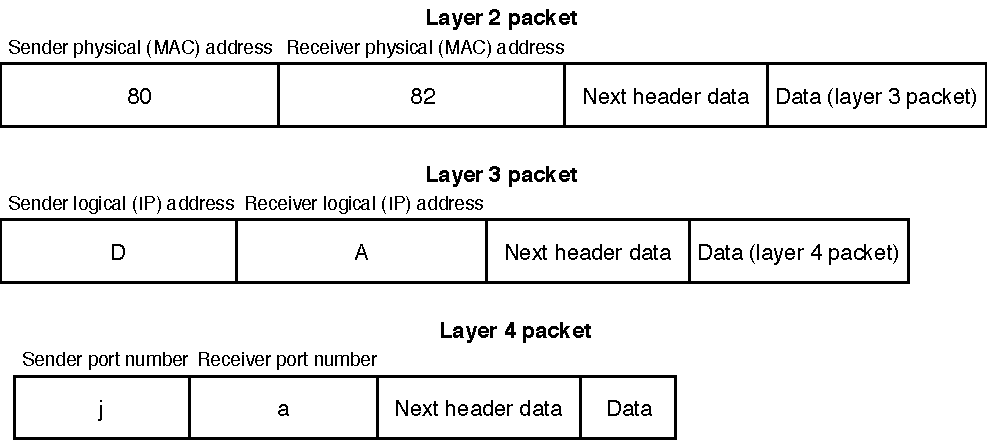
\includegraphics[width=0.7\linewidth]{inc/layer_packets_d_to_a.pdf}
				\caption{Computer D sends data to computer A}
				\label{figure:layer_packets_d_to_a}
			\end{figure}

			Data which sends computer A are encapsulated to layer 4 packet which in addition contains port
			numbers and other header information. Whole layer 4 packet is then encapsulated to layer 3 packet
			which in addition contains logical (IP) addresses and other header information. Finally is whole
			layer 3 packet encapsulated to layer 2 packet which in addition contains physical (MAC) addresses
			and other header information. This layer 2 packet is forwarded to layer 1.

			If the physical destination address of a frame is corrupted during the transmission, the frame will
			be dropped and computer A can be informed about that either when receives this information from device
			that has received this corruption or computer A could waiting for some acknowledgment information which
			has not received.

			Error control mechanisms are still required at layer 4 because sending data are basically divided on multiple
			packets and some of these packets may be dropped, lost or it could be lost their original order and such errors
			could be detected only at layer 4 of receiving side.

		\item % 6.
			TCP in conjunction with IP can ensure the proper message delivery to the destination because TCP operates at
			layer 4 and ensures the reliability of user's message delivery, re-transmit data lost by the lower layers and
			IP operates at layer 3 and is responsible for routing and delivering individual packets.

			Diagram shows relationship between a TCP segment and an IP datagram:
			\begin{figure}[H]
				\centering
				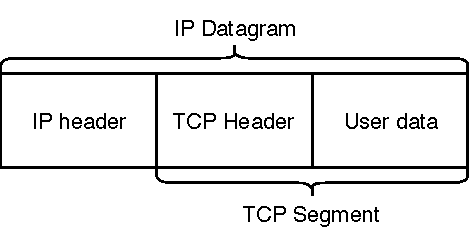
\includegraphics[width=0.4\linewidth]{inc/tcp_ip_relation.pdf}
				\caption{Relationship between a TCP segment and an IP datagram}
				\label{figure:tcp_ip_relation}
			\end{figure}

		\item % 7.
			Diagram of ATM switches:
			\begin{figure}[H]
				\centering
				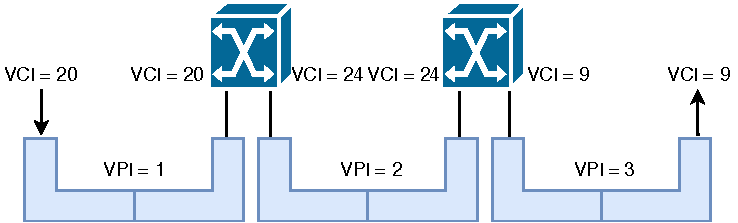
\includegraphics[width=0.7\linewidth]{inc/atm_switch.pdf}
				\caption{ATM switches using both VCI and VPI numbers}
				\label{figure:atm_switch}
			\end{figure}

		\item % 8.
			\textbf{TCP and UDP main differences} -- TCP allows better error checking, more functionality and stability.
			UDP, however, lacks extensive error checking but is considered to be much faster than TCP.
			TCP, unlike UDP, establishes a virtual connection before transmission, guarantees the delivery of data over
			networks and if data is not received correctly, the sending computer will be notified and re-sends the
			information. TCP is connection-oriented protocol and UDP is connection-less protocol.

		\item % 9.
			\textbf{Packet switching} -- Information is divided into a number of specially formatted packets, each of
			which includes some addresses such as logical, physical and port addresses. These packets are routed by a
			series of intermediate nodes of the network to the destination. At the destination, received packets are
			reassembled to form the original stream of data.

			\textbf{Connection-oriented packet switching} -- End-to-end virtual connection to the destination is
			established using single request packet that contains the source and destination addresses. The subsequent
			packets of the same message just need to carry the marking information, which defines the already established
			virtual connection. There is no need to look at addressing information to calculate a path for each packet,
			the intermediate nodes only read the marking information to route the packet to its destination.

			\textbf{Connection-less packet switching} -- Each packet of a message is an independent unit that contains the
			source and destination addresses. Each packet is independently routed at each intermediate nodes it crosses.

		\item % 10.
			Routing table in a connection-less packet switched network \textbf{can not} have two entries with the same destination
			address because this routing table must unambiguously maps destination addresses to output ports.

			Switching table in a connection-oriented packet switched network
			\begin{enumerate}[i)]
				\item \textbf{can} have two entries with the same input VPI, % i)
				\item \textbf{can} have two entries with the same incoming VCI and % ii)
				\item \textbf{can not} have two entries with the same incoming VPI and VCI pair. % iii)
			\end{enumerate}

		\item % 11.
			\textbf{Packet switching} -- End-to-end virtual connection between two devices. Communication connection is always
			available and may be shared by many different users. Messages are split into a number of packets, which will be
			routed and switched separately. Cost-effective, because if no data is being transmitted, there are no transmission
			resources being wasted and bandwidth is shared with many users. Latency and loss of packets are the main concerns.

			\textbf{Circuit switching} -- End-to-end physical connection between two devices. Established before the start of
			a communication section, shared by two users only and remains open for the entire communication section.
			Continuous data flow between two users. Not cost-effective, because stay on the line regardless of the usage
			of that line and bandwidth is no shared. A certain QoS can be guaranteed.

			Addressing mechanisms table:
			\begin{table}[H]
				\centering
				\begin{tabular}{| c | c | c | c |}
					\hline
					& \multicolumn{3}{c |}{\textbf{Communication Stage}} \\ \cline{2-4}
					\multirow{-2}{*}{\textbf{Network Type}} & \textbf{Setup} & \textbf{Data Transmission} & \textbf{Teardown} \\ \hline
					\textbf{Circuit Switching} & end-to-end & \cellcolor{gray} & local \\ \hline
					\textbf{Connection-less Packet Switching} & \cellcolor{gray} & end-to-end & \cellcolor{gray} \\ \hline
					\textbf{Connection-oriented Packet Switching} & end-to-end & local & local \\ \hline
				\end{tabular}
				\caption{Addressing mechanisms}
				\label{table:addressing_mechanisms}
			\end{table}

		\item % 12.
			Frame Relay can operate in a multi-protocol environment because it handles all protocols. It simply encapsulates another
			protocol into a Frame Relay envelope and carries it through the network.

		\item % 13.
			\textbf{X.25:}
			\begin{description}
				\item
					Payload error control -- Tight error control on every packet at every intermediate node.

				\item
					Latency -- Large delay time. Error control increases transmission delay.

				\item
					Packet size -- Relatively small packet size (128 bytes or 256 bytes long).

				\item
					Data transmission capacity -- Operates at very low speeds ranging from 56\,kb/s to 2\,Mb/s.

				\item
					Types of traffic supported -- For low speed data transmission only.
			\end{description}

			\textbf{Frame Relay:}
			\begin{description}
				\item
					Payload error control -- The intermediate nodes does not correct data errors. Error control at endpoints of networks.

				\item
					Latency -- Delay is reduced because the intermediate nodes does not correct data errors. Latency still could be a
					problem due to large packet size.

				\item
					Packet size -- Large packet size (up to 9\,000 bytes and variable).

				\item
					Data transmission capacity -- Operates at a higher speed (45\,Mb/s).

				\item
					Types of traffic supported -- Possible to carry voice and video.
			\end{description}

			\textbf{Asynchronous Transfer Mode (ATM):}
			\begin{description}
				\item
					Payload error control -- No payload error checking is made in the core of the networks. Payload error control
					at endpoints.

				\item
					Latency -- Latency is reduced due to uniform packet size. Time delay is minimized because no payload error
					checking is made in the core of the networks, routing time at each node across networks is minimizing and
					switching can be performed by hardware.

				\item
					Packet size -- Uniform 53-byte packet (5 bytes for addressing information and 48 bytes for payload).

				\item
					Data transmission capacity -- Speed can be very high (10\,Gb/s to 160\,Gb/s, Tb/s for some new products).

				\item
					Types of traffic supported -- Suitable for real-time traffic. Carries voice, data, multimedia, images, and
					other forms of traffic, so it is suitable for all kinds of traffic.
			\end{description}

		\item % 14.
			\textbf{Physical layer} -- Provides the physical transportation of cells across network. It carries ATM cells rather
			than individual bits. These cells are multiplexed with other traffic for transmission.
			Physical layer defines transmission media, transmission rate, physical interface and coding schemes.

			\textbf{ATM layer} -- Switches the cells around the network based on routing information. ATM layer provides routing,
			traffic management, switching and multiplexing services. Process outgoing traffic by accepting 48-byte segments from
			the AAL sub-layers and transforming them into 53-byte cells by adding a 5-byte header.

			\textbf{ATM adaptation layer (AAL)} -- Assembles and disassembles broadband services into a stream of cells. The native
			traffic stream goes through the ALL, where it is segmented into 48-byte cells. ALL accepts any type of payload, both
			data frames and continuous stream of bits. AAL uses two sub-layers: the convergence sub-layer (CS) which guarantees
			the integrity of the data and the segmentation and reassembly sub-layer (SAR) where assembles and disassembles is
			performed. ATM defines four versions of the AAL: AAL1, AAL2, AAL3/4 and AAL5.

		\item % 15.
			\begin{enumerate}[i)]
				\item % i)
					\textbf{1} padding byte is required. \textbf{1\,087} data units are passed from SAR sub-layer to ATM layer.
					\textbf{1\,087} ATM cells are produced.

				\item % ii)
					Minimum number of ATM cells produced from an input packet may be \textbf{1} and maximum number may be \textbf{1\,490}.

				\item % iii)
					The value of \texttt{Btag} is repeated in each cell to identify all the cells belonging to the same packet. The value is
					the same as the value of \texttt{Etag}.
					So if there are 47\,787 bytes of data, then the same \texttt{Btag/Etag} is repeated \textbf{2\,174 times} and for
					maximum number of ATM cells, the same \texttt{Btag/Etag} is repeated \textbf{2\,980 times}.

				\item % iv)
					\textbf{LI (length indicator)} in CS header is the 6-bit field indicates how much of the final packet is data.
					\textbf{SF (start field)} in SAR header defines the offset from the beginning of the packet.
			\end{enumerate}

		\item % 16.
			\textbf{Baseband transmission} -- Transmits a digital signal directly through a cable, thus one signal is allowed
			at any given time. It is less expensive to implement but capacity and transmission length is limited.

			\textbf{Broadband transmission} -- Signals are transmitted using carrier waves of different frequencies, thus
			multiple signals are allowed to transmit simultaneously. It is more expensive to purchase and maintain but
			bandwidth and length of transmission is not so limited.

			\textbf{Topologies usage} -- The \textbf{tree} topology is commonly used in broadband LANs and the \textbf{bus},
			\textbf{ring} and \textbf{star} topologies are used in basedband LANs

		\item % 17.
			Most common LAN topologies diagrams:
			\begin{figure}[H]
				\begin{minipage}{0.5\linewidth}
					\centering
					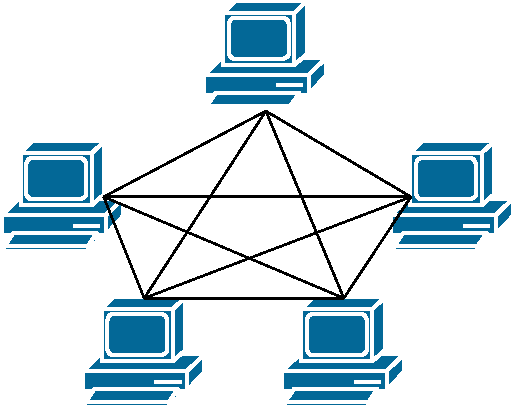
\includegraphics[width=0.8\linewidth]{inc/mesh_topology.pdf}
					\caption{Mesh topology}
					\label{figure:mesh_topology}
				\end{minipage}
				\begin{minipage}{0.5\linewidth}
					\centering
					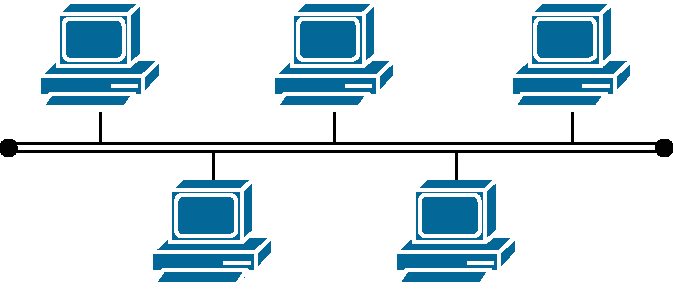
\includegraphics[width=0.8\linewidth]{inc/bus_topology.pdf}
					\caption{Bus topology}
					\label{figure:bus_topology}
				\end{minipage}
			\end{figure}
			\begin{figure}[H]
				\begin{minipage}{0.5\linewidth}
					\centering
					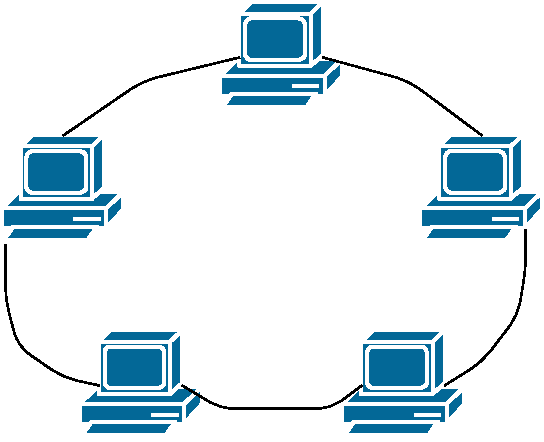
\includegraphics[width=0.8\linewidth]{inc/ring_topology.pdf}
					\caption{Ring topology}
					\label{figure:ring_topology}
				\end{minipage}
				\begin{minipage}{0.5\linewidth}
					\centering
					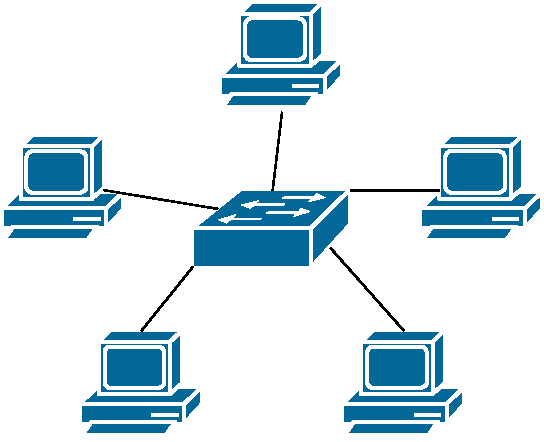
\includegraphics[width=0.8\linewidth]{inc/star_topology.pdf}
					\caption{Star topology}
					\label{figure:star_topology}
				\end{minipage}
			\end{figure}

			\textbf{Tree topology} -- The tree topology has a root node, which forms the base of the network. The root node then communicates
			with a number of smaller nodes, and those in turn communicate with an even greater number of smaller nodes. Tree topology is
			actually combination of star and bus topology. Tree topology has binary tree structure. All transmission must pass through
			the root node.
	\end{enumerate}


\end{document}
